\documentclass{article}
\usepackage{color}
\usepackage{graphicx}

%\usepackage{enumerate}
\usepackage{graphicx}
\usepackage{color}
\usepackage[cmex10]{amsmath}
\usepackage{array}
\usepackage{float}
\usepackage[utf8]{inputenc} 
\usepackage[portuguese]{babel}
\usepackage[font=normalsize,format=plain,labelfont=bf,up,textfont=up,figurename=Figura,tablename=Tabela]{caption}
\usepackage{subcaption}
\usepackage[top=1in, bottom=1in, left=1.25in, right=1.25in]{geometry}
\usepackage{indentfirst}
\usepackage{fancyhdr}

%% LaTeX Draw
%
%\usepackage[usenames,dvipsnames]{pstricks}
%\usepackage{epsfig}
%\usepackage{pst-grad} % For gradients
%\usepackage{pst-plot} % For axes
%\usepackage[space]{grffile} % For spaces in paths
%\usepackage{etoolbox} % For spaces in paths
%\makeatletter % For spaces in paths
%\patchcmd\Gread@eps{\@inputcheck#1 }{\@inputcheck"#1"\relax}{}{}
%\makeatother

% Font packages
\usepackage{amssymb}
\usepackage{amsfonts}
\usepackage{steinmetz}
% Nice extra font package, e.g. \mathds{1}
\usepackage{dsfont}


% Use multiple rows when writing tables
\usepackage{multirow}
\usepackage{booktabs}
\usepackage{bigstrut}
    \setlength\bigstrutjot{3pt}

% Uncomment next line to make footnots per page
\usepackage{perpage}

% Uncoment next group of lines to create the table of contents for the PDF
\usepackage{hyperref}
\definecolor{darkblue}{rgb}{0,0,0.5}
\hypersetup{
    pdftitle={Trabalho 1},
    pdfauthor={Gabriel Pelielo},
    bookmarksnumbered=true,     
    bookmarksopen=true,         
    bookmarksopenlevel=1,       
    colorlinks=true,
    linkcolor=darkblue,
    filecolor=darkblue,  
    urlcolor=darkblue,  
    citecolor=darkblue,              
    pdfstartview=Fit,           
    pdfpagemode=UseOutlines,    % this is the option you were lookin for
    pdfpagelayout=TwoPageRight
}

\renewcommand{\title}{Trabalho 2}
\newcommand{\subtitle}{Introdução à Otimização}
\pagestyle{fancy}
\fancyhead[L]{\title}
\fancyhead[R]{\subtitle}
\fancyhead[C]{\thepage}
\fancyfoot[C]{}

\allowdisplaybreaks

\renewcommand{\labelitemi}{\scalebox{0.8}[0.8]{$\bullet$}}
\newcommand{\tab}{\hspace{0.5cm}}

\definecolor{lightyellow}{rgb}{1,0.9568,0.8039}
\definecolor{mygreen}{rgb}{0, 0.35, 0}
\definecolor{myblue}{rgb}{0,0,1}

\begin{document}
\large
\begin{titlepage}
\begin{center}

% Upper part of the page. The '~' is needed because \\
% only works if a paragraph has started.

\includegraphics[width=0.15\textwidth]{logo.png}%~\\[0.5cm]

% Title
\rule{\linewidth}{0.5mm} \\[0.4cm]
{ \huge \bfseries \title \\[0.4cm] }
\rule{\linewidth}{0.5mm} \\[0.5cm]

\textsc{\Large \subtitle}\\[1.5cm]

% Author and supervisor
\begin{minipage}{0.4\textwidth}
\begin{flushleft} \large
\textbf{Alunos: \newline Cayo Valsamis \newline Gabriel Pelielo \newline Rafael Accácio \newline Rodrigo Moysés}\\
%NOME DOS ALUNOS

\end{flushleft}
\end{minipage}
\begin{minipage}{0.4\textwidth}
\begin{flushright} \large
\textbf{Professor:\newline Afonso Celso del Nero \newline \newline \newline} \\
%NOME DO PROFESSOR
\end{flushright}
\end{minipage}

\vfill

% Bottom of the page
{\large \today}

\end{center}
\end{titlepage}

\tableofcontents

\newpage

\section{Introdução}

O trabalho detalhado neste relatório se baseia em analisar métodos numéricos para realizar busca de mínimos de funções vetoriais. Foram implementados cinco métodos diferentes de localização de mínimos:

\begin{itemize}
	\item Método da Descida Máxima (ou gradiente)
	\item Método do Gradiente Conjugado
	\item Método de Newton
	\item Método de Newton Modificado
	\item Método de Quase Newton
\end{itemize}

Todos os métodos foram implementados na plataforma \textit{MATLAB}, através de um programa de interface gráfica usado para escolher o método desejado e inserir alguns valores necessários para executar a busca. O objetivo do trabalho foi comparar esses métodos de acordo com os quesitos de tempo de execução, número necessário de iterações e por fim qualificá-los de acordo com cada função inserida.

\section{Método da Descida Máxima}\label{sec:descida_max}

O método de Descida máxima, ou método do gradiente, se baseia em um método muito simples para encontrar o mínimo de uma função.
 A partir de um ponto inicial calcula-se a direção de maior de crescimento, de descida máxima ou sentido inverso do gradiente, que dão nome ao método, 
e faz-se um avanço nessa mesma direção.\\
 
Como sabemos, o gradiente de uma função representa sua direção de maior crescimento. Sabendo disso utiliza-se a direção oposta, 
mas a questão que fica é qual o avanço é necessário. Para resolver isso, a direção do gradiente foi normalizada, $d^k$, e criou-se uma variável, $\alpha$, que indica o avanço a ser feito. 

Com o gradiente calculado naquele ponto, usa-se um método de minimização unidimensional qualquer para minimizar a função $x^k - \alpha d^k$. 
Foi escolhido o método da seção áurea, devido a sua grande flexibilidade e por encontrar o mínimo com poucas iterações e baixo esforço computacional. 
Após a minimização utilizamos o valor de $\alpha$ que a minimiza como avanço.
\\
Dessa forma faz-se a iteração para encontrar o próximo ponto, que a princípio 
está mais perto do mínimo. E assim faz-se até convergir ao ponto de mínimo da função (considerando que a mesma o possui).

Como métodos de parada foram escolhidos o tamanho da norma do vetor diferença de gradiente em cada iteração, a norma entre a diferença entre os pontos em cada iteração e finalmente o número de iterações.

Para verificar a convergência do método vemos como são as direções de avanço do algoritmo e também sua norma. Sabe-se a partir de \cite{Notastioafel} que cada iteração tem direção perpendicular a anterior e que a convergência dá-se quando cada avanço é menor que o anterior, assim como vemos na figura \ref{fig:stegradeszigzag}


\begin{figure}[H]
	\begin{center}
		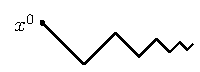
\includegraphics[width=8cm]{../tikz/stegrades}  
		\caption{Representação do avanço convergente em zig-zag com ângulos retos.}
		\label{fig:stegradeszigzag}
	\end{center}
\end{figure}


	\begin{quote}
		\centering
		Lei de Iteração:
	\end{quote}

\begin{equation}
	x^{k+1} = x^k - \alpha d^k
	\end{equation}
	
Após construir o algoritmo, foram feitos testes usando algumas funções:

\begin{itemize}
	\item $ f_1(x,y) = x^2 + y^2$
	\item $ f_2(x,y) = -e^{-x^2 -y^2}$
	\item $ f_3(x,y) = cos(\frac{xy}{5})+sin(\frac{xy}{5}) $
	\item $ f_4(x,y) = |x+y| $
\end{itemize}


\newpage

\begin{figure}[H]
	\begin{center}	
		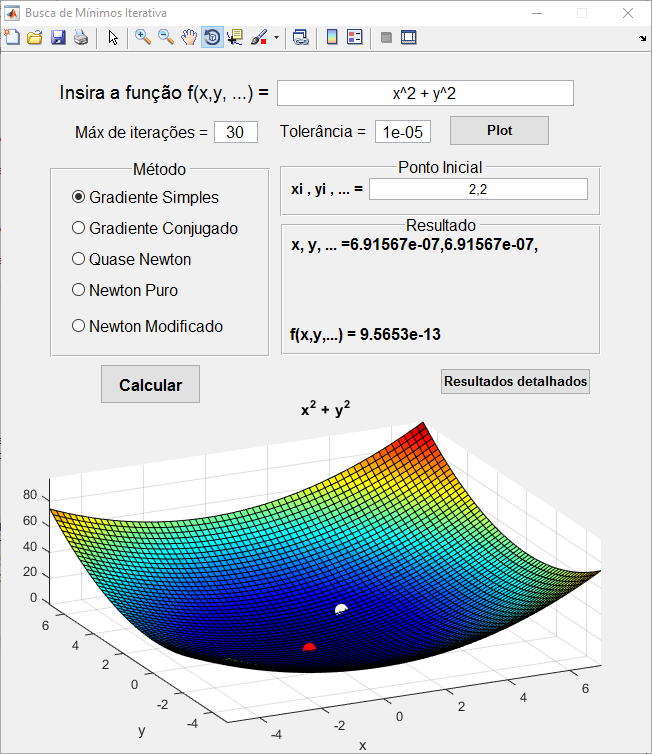
\includegraphics[width=12cm]{../stegrades/f1_gui.PNG}
		\caption{Janela de inicialização de $ f_1(x,y) $}
		\label{fig:f1_gui}
	\end{center}
\end{figure}



\begin{figure}[H]
	\begin{center}	
		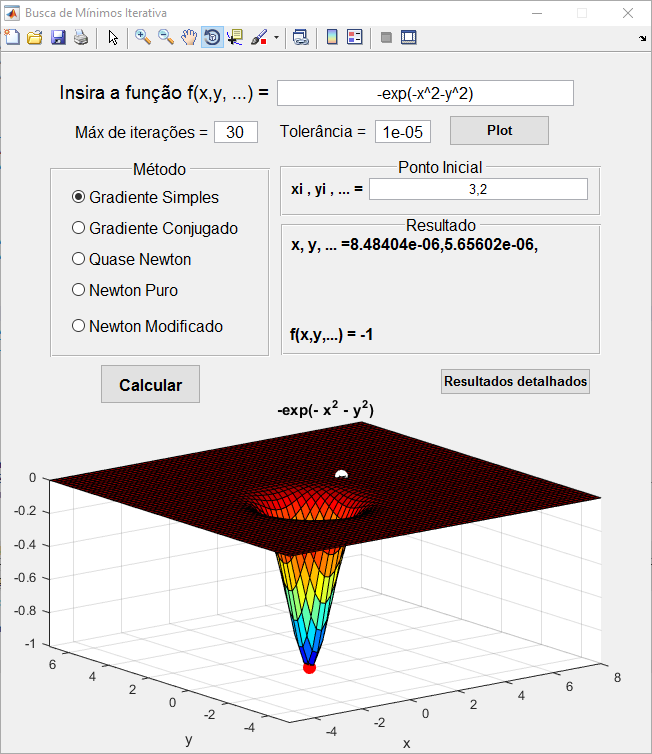
\includegraphics[width=12cm]{../stegrades/f2_gui.PNG}
		\caption{Janela de inicialização de $ f_2(x,y) $}
		\label{fig:f2_gui}
	\end{center}
\end{figure}



\begin{figure}[H]
	\begin{center}	
		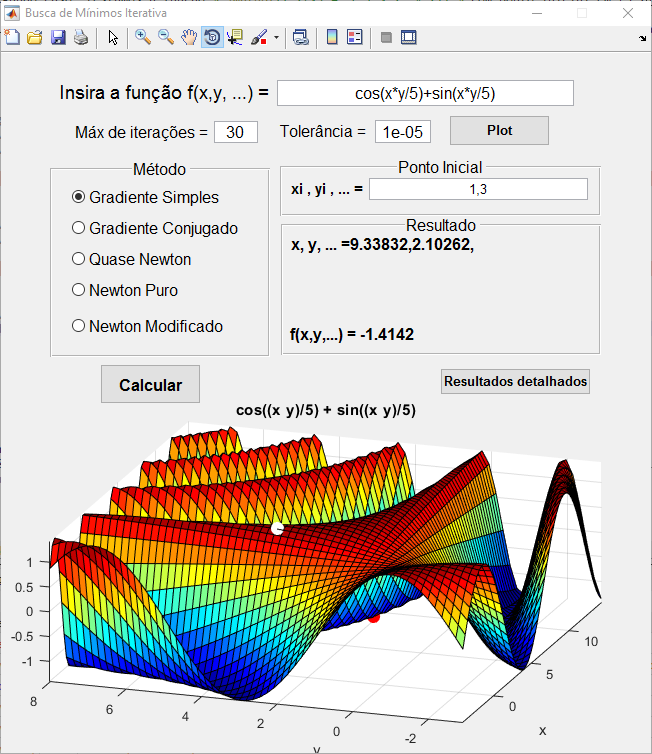
\includegraphics[width=12cm]{../stegrades/f3_gui.PNG}
		\caption{Janela de inicialização de $ f_3(x,y) $}
		\label{fig:f3_gui}
	\end{center}
\end{figure}



\begin{figure}[H]
	\begin{center}	
		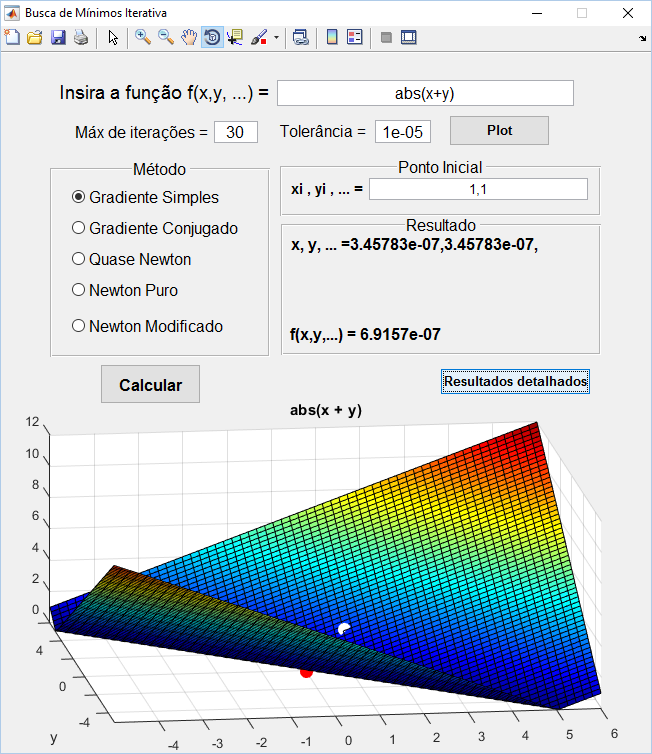
\includegraphics[width=12cm]{../stegrades/f4_gui.PNG}
		\caption{Janela de inicialização de $ f_4(x,y) $}
		\label{fig:f4_gui}
	\end{center}
\end{figure}






\newpage





\section{Método do Gradiente Conjugado}\label{sec:grad_conj}

O método do Gradiente Conjugado nada mais é do que um ajuste sobre o método do Gradiente descrito na seção \ref{sec:descida_max}. As mudanças de direção abruptas, conforme ilustrado na figura \ref{fig:stegradeszigzag}, são suavizadas com a adição do coeficiente de inércia $\beta$, que conserva uma fração da direção anterior. Assim, a direção de avanço toma a seguinte forma:
	\begin{equation}
	d^{k+1} = -g(x^{k+1}) + \beta_k d^k
	\end{equation}
A Lei de Iteração é a mesma do método do Gradiente:
		\begin{align}
			x^{k+1} &= x^k + \alpha_k d^k \\
			\tilde{f}(\alpha) &= f(x^k + \alpha d^k)
		\end{align}
A função $\tilde{f}(\alpha)$ é minimizada utilizando a razão áurea.\\
Já o coeficiente $\beta$ é uma relação entre o gradiente atual e o anterior.\\
		Segundo \textit{Polak-Rebière}:
		\begin{equation}
			\beta_k = \frac{||g^{k+1}|| - [g^+1]^T g^k}{||g^k||}
		\end{equation}
Com essa suavização das direções de avanço, é esperado que esse método convirja com menos iterações do que o método do Gradiente. 

Depois de construído o algoritmo, foram testadas quatro funções para efeitos de comparação:

\begin{itemize}
	\item $ f_1(x,y) = x^2 + y^2$
	\item $ f_2(x,y) = -e^{-x^2 -y^2}$
	\item $ f_3(x,y) = cos(\frac{xy}{5})+sin(\frac{xy}{5}) $
	\item $ f_4(x,y) = |x+y| $
\end{itemize}

\begin{figure}[H]
	\begin{center}
		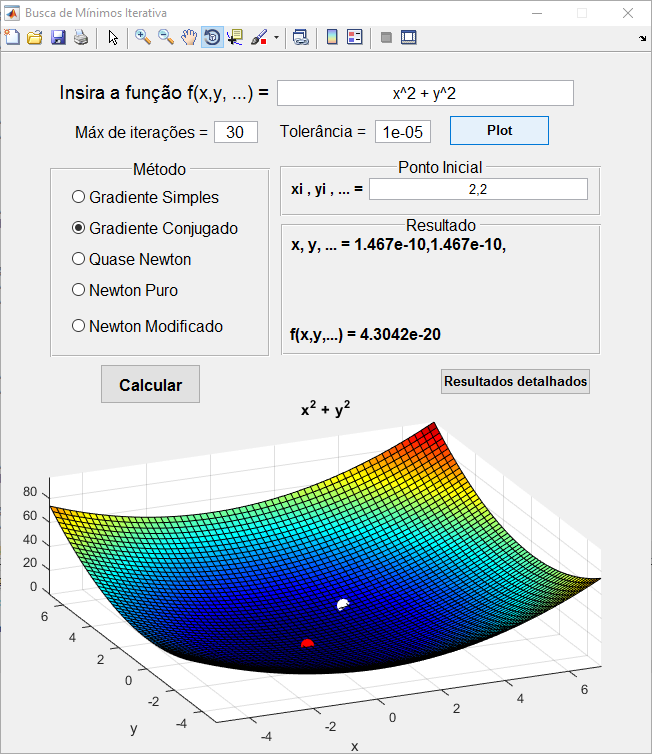
\includegraphics[width=12cm]{../gradiente_conjugado/f1_gui}   
		\caption{Janela de inicialização de $ f_1(x,y) $}
		\label{fig:gradiente_conjugado_f1_gui}
	\end{center}
\end{figure}

\begin{figure}[H]
	\begin{center}
		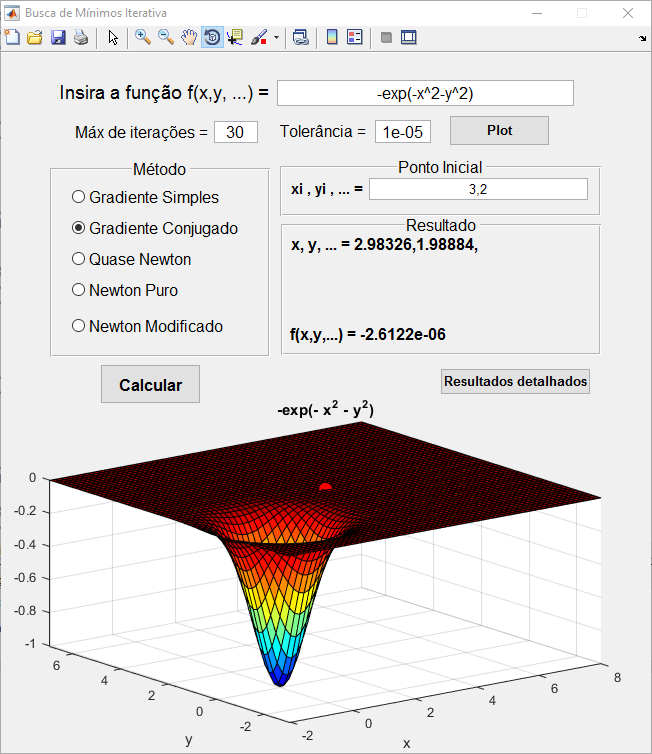
\includegraphics[width=12cm]{../gradiente_conjugado/f2_gui}   
		\caption{Janela de inicialização de $ f_2(x,y) $}
		\label{fig:gradiente_conjugado_f2_gui}
	\end{center}
\end{figure}

\begin{figure}[H]
	\begin{center}
		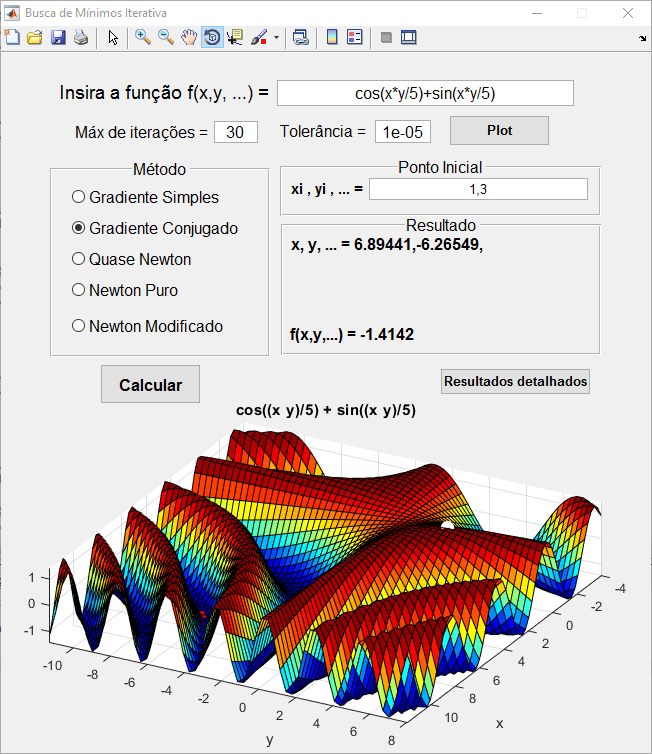
\includegraphics[width=12cm]{../gradiente_conjugado/f3_gui}   
		\caption{Janela de inicialização de $ f_3(x,y) $}
		\label{fig:gradiente_conjugado_f3_gui}
	\end{center}
\end{figure}


\begin{figure}[H]
	\begin{center}
		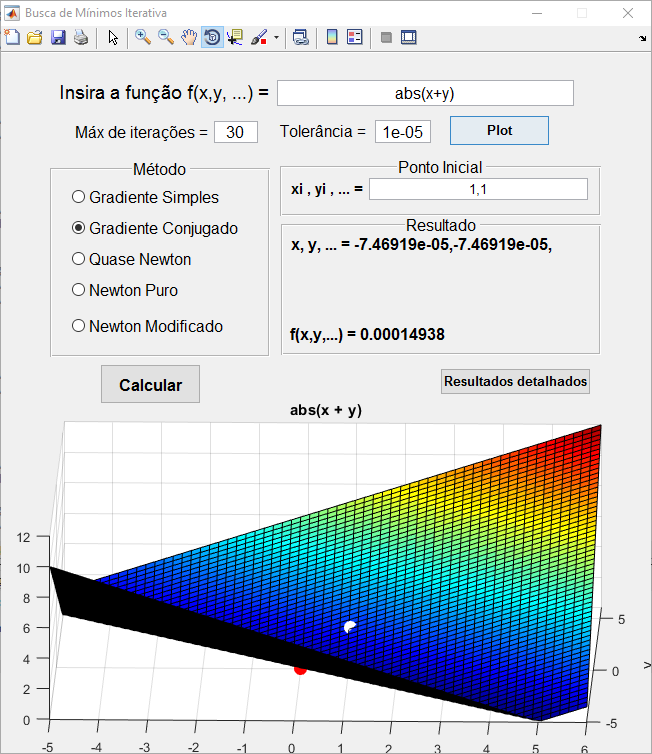
\includegraphics[width=12cm]{../gradiente_conjugado/f4_gui}   
		\caption{Janela de inicialização de $ f_4(x,y) $}
		\label{fig:gradiente_conjugado_f4_gui}
	\end{center}
\end{figure}


\section{Método de Newton}\label{sec:newton}

Os métodos de Newton se baseiam em encontrar uma aproximação quadrática $ q(x) $ a partir do teorema de Taylor para a função objetivo $ f(x) $, e assim, encontrar o seu mínimo.
	
	\begin{quote}
		\centering
		Lei de Iteração:
	\end{quote}
	
	\begin{equation}
		x^{k+1} = x^k - [G^k]^{-1}g^k
	\end{equation}

Teoricamente, a vantagem do método de Newton em relação aos outros é que, para funções quadráticas, ele converge em apenas uma iteração. Porém, um dos problemas do método é ele ser de segunda ordem, o que significa que ele depende tanto do valor da hessiana quanto do gradiente da função objetivo, e alguns casos, a convergência pode ser comprometida devido ao fato de que a hessiana em um dado ponto pode não ser positiva definida.

Depois de construído o algoritmo, foram testadas quatro funções para efeitos de comparação:

\begin{itemize}
	\item $ f_1(x,y) = x^2 + y^2$
	\item $ f_2(x,y) = -e^{-x^2 -y^2}$
	\item $ f_3(x,y) = cos(\frac{xy}{5})+sin(\frac{xy}{5}) $
	\item $ f_4(x,y) = |x+y| $
\end{itemize}

\newpage

\begin{figure}[H]
	\begin{center}
		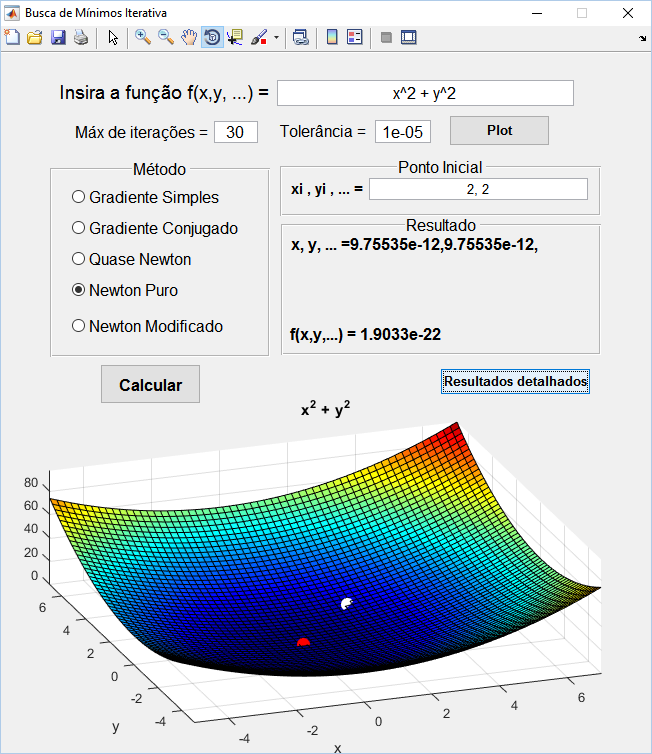
\includegraphics[width=12cm]{../newton/f1_gui}   
		\caption{Janela de inicialização de $ f_1(x,y) $}
		\label{fig:newton_f1_gui}
	\end{center}
\end{figure}

\begin{figure}[H]
	\begin{center}
		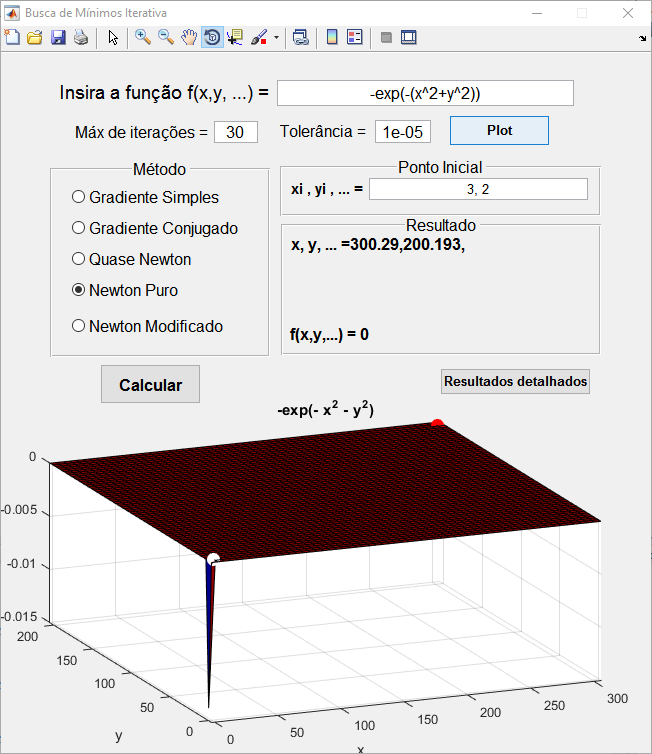
\includegraphics[width=12cm]{../newton/f2_gui}   
		\caption{Janela de inicialização de $ f_2(x,y) $}
		\label{fig:newton_f2_gui}
	\end{center}
\end{figure}

\begin{figure}[H]
	\begin{center}
		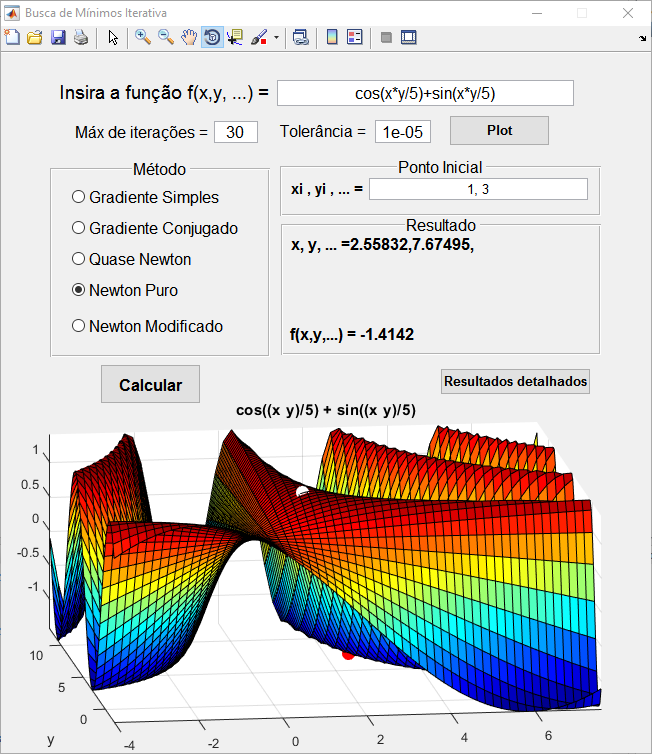
\includegraphics[width=12cm]{../newton/f3_gui}   
		\caption{Janela de inicialização de $ f_3(x,y) $}
		\label{fig:newton_f3_gui}
	\end{center}
\end{figure}


\begin{figure}[H]
	\begin{center}
		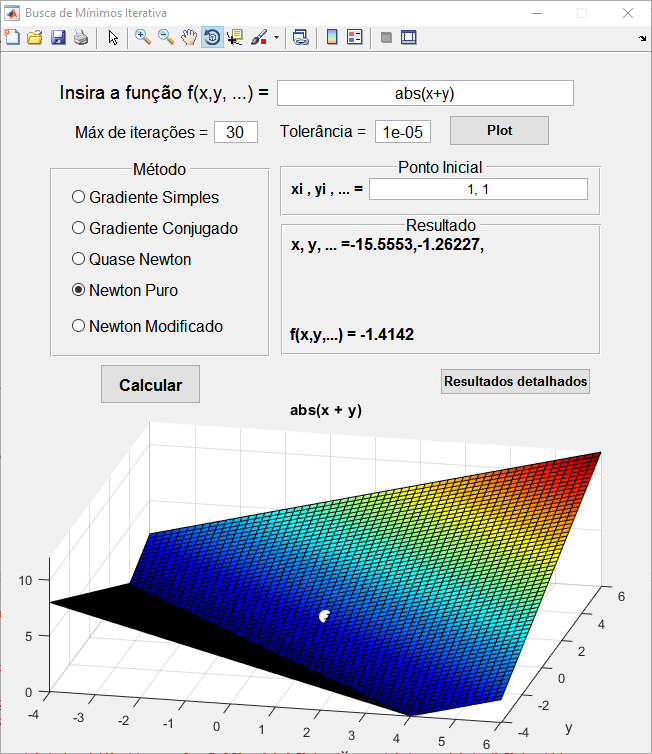
\includegraphics[width=12cm]{../newton/f4_gui}   
		\caption{Janela de inicialização de $ f_4(x,y) $}
		\label{fig:newton_f4_gui}
	\end{center}
\end{figure}


\section{Método de Newton Modificado}\label{sec:newton_mod}

\begin{frame}{Newton Modificado}
	
	Para melhorar o método de Newton, foram feitas algumas alterações, como:
	
	\begin{itemize}
		\item Diminuição do avanço na direção $ d^k $, da forma:
	\end{itemize}
	
	\begin{equation}
	x^{k+1} = x^k + \alpha_k d^k
	\end{equation}
	
	onde $ \alpha_k $ minimiza $ \tilde{f}(\alpha) = f(x^k + \alpha d^k) $
	
\end{frame}


\begin{frame}{Newton Modificado}
	
	\begin{itemize}
		\item Correção do sinal da Hessiana por um truque matricial:
	\end{itemize}	
	
	\begin{equation}
	F^k = G^k + \gamma I_n
	\end{equation}
	
	Em que $ F^k $ tem autovalores positivos para poder gerar uma direção $ d^k $ de descida da forma
	
	\begin{equation}
	d^k = -[F^k]^{-1}g^k = -[\nabla^2 f(x^k) + \gamma I_n]^{-1}\nabla f(x^k)
	\end{equation}
	
\end{frame}

\section{Método de Quase Newton}\label{sec:quase_newton}

\begin{frame}{Método de Quase Newton}
	Todos os métodos de Newton baseiam-se em facilitar o cálculo da Hessiana. O método de Quase Newton diferencia-se por apoiar-se na chamada "Condição de Quase Newton":
	\\
	\begin{equation}
		H^{k+1} \gamma^{k} = \delta^{k} = \left\{
		\begin{tabular}{c}
		\gamma^{k} = g^{k+1} - g^{k}\\
		\delta^{k} = x^{k+1} - x^{k} 
		\end{tabular}
	\end{equation}
\end{frame}

\begin{frame}	
Duas possibilidades para se gerar matrizes H satisfazendo essa restrição são o método de Davidon-Fletcher-Powell (DFP):
\begin{equation}
	H^{k+1} = H - \frac{H \gamma \gamma^T H}{\gamma^T H \gamma} + \frac{\delta \delta^T}{\delta^T \gamma}
\end{equation}	

ou o método de Broyden-Fletcher-Goldfarb-Shanno (BFGS)

\begin{equation}
H^{k+1} = H - \frac{\delta \gamma^T H + H \gamma \delta^T}{\delta^T \gamma} + \Bigg( 1 + \frac{\gamma^T H \gamma}{\delta^T \gamma}\Bigg) \frac{\delta \delta^T}{\delta^T \gamma}
\end{equation}	


\end{frame}

\section{Conclusão}

bla bla bla
	
%\textcolor{mygreen}{text} - Dá cor verde ao texto
%\textcolor{myblue}{text}  - Dá cor azul  ao texto
\bibliographystyle{plain}
\bibliography{bibliografia}

\end{document}